\documentclass[10pt,twocolumn]{article}
\usepackage[margin=0.75in]{geometry}
\usepackage{graphicx,booktabs,xcolor,amssymb,amsmath}
\usepackage[colorlinks=true,linkcolor=teal,citecolor=teal,urlcolor=teal]{hyperref}
\usepackage{titlesec}
\definecolor{ink}{HTML}{1F2A37}
\definecolor{teal}{HTML}{0D9488}
\titleformat{\section}{\large\bfseries\color{ink}}{\thesection}{0.6em}{}
\titleformat{\subsection}{\normalsize\bfseries\color{ink}}{\thesubsection}{0.5em}{}
\setlength{\parskip}{3pt}\setlength{\parindent}{0pt}
\newcommand{\R}{\textcolor{teal}}

\title{\vspace{-1.5em}\textbf{\color{ink}ToothPrint: A Certified, Partial-Overlap-Robust System\\for Dental Biometric Identification}}
\author{Krishi Attri\\\small Independent research \quad\textbar\quad \texttt{kattri@snu.ac.kr} \quad\textbar\quad \href{https://github.com/Archerkattri/toothprint}{github.com/Archerkattri/toothprint}}
\date{\vspace{-1em}\small Methods report. Every number is reproduced by a committed script + result JSON; every limitation is stated.}

\begin{document}
\twocolumn[
\maketitle
\begin{abstract}
\noindent The dental arch is an individual ``tooth print'': crown contours, cusp geometry, the gingival margin, and the pattern of restorations. We assemble a dental-identity system that (i) recognises a person from a 3D intraoral scan or a 2D radiograph, (ii) returns a \textbf{certified} accept/abstain decision with a distribution-free false-match-rate bound, and (iii) is \textbf{robust to partial overlap}---the missing-teeth query where prior rigid methods collapse. Our contributions are a learned point-correspondence matcher that lifts 50\%-tooth-loss identification from 0.23 (rigid GICP) to \textbf{0.87}, a conformal open-set decision hardened against look-alikes, a restoration biometric demonstrated on both CBCT and plain radiographs, and an honest characterisation: full DET curves, ablations, a cross-dataset domain-gap measurement, and the regimes where the system must abstain. The one limit no method here closes is real cross-session data. \vspace{0.5em}
\end{abstract}
]

\section{Introduction}
Forensic and clinical dental identification is classically manual (charting) or, recently, rigid 3D scan registration. Two gaps persist: (a) no \emph{certificate}---methods report Rank-N accuracy but never a finite-sample bound on the false-match rate of an individual verdict; and (b) \emph{partial overlap}---a query arch missing teeth (extraction, trauma, field-of-view) breaks the rigid alignment that all registration methods depend on. ToothPrint targets both, and treats honesty about failure regimes as a first-class deliverable.

\section{Related work and positioning}
The only dedicated 3D-intraoral identity pipeline with proper Rank-1 is \textbf{Zhou et al. 2024} (\emph{Bioengineering})---FPFH + SAC-IA + ICP + RMSE, the same registration family as our geometric core---reporting Rank-1 100\% on 160 real adults with $\sim$1-year re-scans (closed-set, private data). We match its saturated accuracy (Rank-1 0.995 / EER 0.5\% on 200 arches) and \textbf{lead on a certified, bounded-FMR decision with open-set rejection} that no prior dental work reports, and on \textbf{learned partial-overlap correspondence}, which the registration literature lacks for this domain. ToothPrint's defensible lane is \emph{certification + partial-overlap robustness}, not a higher saturated number.

\section{Methods}
\textbf{Geometric identity (3D).} A query re-scan is given its best \emph{rigid} fit to each gallery arch---PCA principal-axis initialisation (four proper-rotation hypotheses; robust to the self-similar palate that defeats FPFH) refined by multi-scale Generalised-ICP---and scored by mean point-to-surface distance. Rigid (no scale) so the score is shape, not pose.

\textbf{Learned embedding.} A DGCNN (EdgeConv) encoder with a sub-centre ArcFace head maps an arch to an L2-normalised descriptor. \emph{Crop-hardening}: training with aggressive partial crops (keep $\geq 0.35$) makes the descriptor coverage-robust at no full-coverage cost.

\textbf{Learned point correspondence (CorrNet).} The key partial-overlap result. A DGCNN backbone emits a \textbf{unit descriptor per point}, trained with an InfoNCE correspondence loss---cropping a canonical point set yields ground-truth point matches for free. At test, a partial query is matched point-to-point against each gallery arch (mutual nearest-neighbours $\rightarrow$ weighted Procrustes), and the residual over \emph{all} query points scores the fit.

\textbf{Conformal certificate.} Calibrating a threshold on held-out genuine / nearest-impostor scores yields an empirical false-match rate $\leq \alpha$, distribution-free and finite-sample.

\textbf{Unified decision.} Retrieve by embedding (recall) $\rightarrow$ verify the shortlist by CorrNet correspondence (precision) $\rightarrow$ accept above the conformal threshold, else \textbf{abstain}.

\textbf{Multimodal \& dental-work.} On paired CBCT+IOS, three independent biometrics---IOS crowns, CBCT bone/root geometry, CBCT restoration cloud (HU $>2500$)---are scored and fused. The restoration pattern also extends to 2D radiographs via a per-tooth local-contrast extractor (a restoration is the patch far brighter than its own tooth's median).

\section{Datasets and protocols}
Poseidon3D (intraoral STL, 200: 150 train / 50 held-out), Teeth3DS+ (intraoral OBJ, 150, cross-dataset), DenPAR (periapical radiographs, 400 / 165 restoration-bearing), Figshare CBCT+IOS (paired, 55). All are single-timepoint, so \textbf{genuine queries are synthetic}---acquisition repositioning, sensor noise, and partial crops (planar or realistic whole-tooth dropout). This is disclosed on every result and is the central limitation (\S7).

\section{Results}
\textbf{Identity (full coverage).} 3D Rank-1 \textbf{0.995} (N=200, EER 0.5\%, AUC 0.997, fidelity 0.05\,mm); 2D Rank-1 \textbf{1.000} (N=400, EER 0). Conformal empirical FMR tracks $\alpha$ in every ablation. Fig.~\ref{fig:det} gives full DET curves---a first for dental identity.

\textbf{Partial overlap (the contribution).} Table~\ref{tab:partial} and Fig.~\ref{fig:panel} (top-left): under realistic whole-tooth dropout, CorrNet lifts keep-0.5 from 0.23 (GICP) to \textbf{0.87}. An \emph{untrained} CorrNet already scores 0.70---so the gain is $\sim$half the correspondence-plus-rigid-verification \emph{architecture} and $\sim$half the \emph{learned} descriptors. Honest correction kept: planar-crop numbers were optimistic vs realistic dropout (keep-0.3 $0.80\!\rightarrow\!0.57$).

\begin{table}[t]\centering\small
\begin{tabular}{lcc}\toprule
method & keep-0.5 & keep-0.3 \\\midrule
rigid GICP & 0.23 & 0.10 \\
crop-hardened embedding & 0.64 & 0.26 \\
\textbf{CorrNet (realistic dropout)} & \textbf{0.87} & \textbf{0.57} \\
CorrNet (planar crop) & 0.91 & 0.80 \\\bottomrule
\end{tabular}
\caption{Rank-1 under tooth loss, held-out unseen subjects.}\label{tab:partial}
\end{table}

\textbf{Multimodal fusion.} On 55 paired patients: IOS 1.000, CBCT-bone 0.945, dental-work 0.927. In a degraded regime the \textbf{oracle bound is 1.000} (modalities complementary), naive equal-weight fusion \emph{hurts} (dilution), and quality-weighted fusion beats the best single (0.867 vs 0.833)---a real but Rank-1-only gain (its AUC regresses).

\textbf{Dental-work on 2D radiographs.} Per-tooth local contrast (global thresholding fails on over-saturated JPEGs) identifies 165 subjects at Rank-1 \textbf{0.91--0.99} (robust to jitter + a dropped restoration; chance 0.006).

\textbf{Unified certified decision.} Full coverage FNIR@FMR=1\% $= 0.00$; partial (keep-0.5) 0.74---best of all methods but does not escape the open-set ceiling (\S6), so it abstains.

\begin{figure}[t]\centering
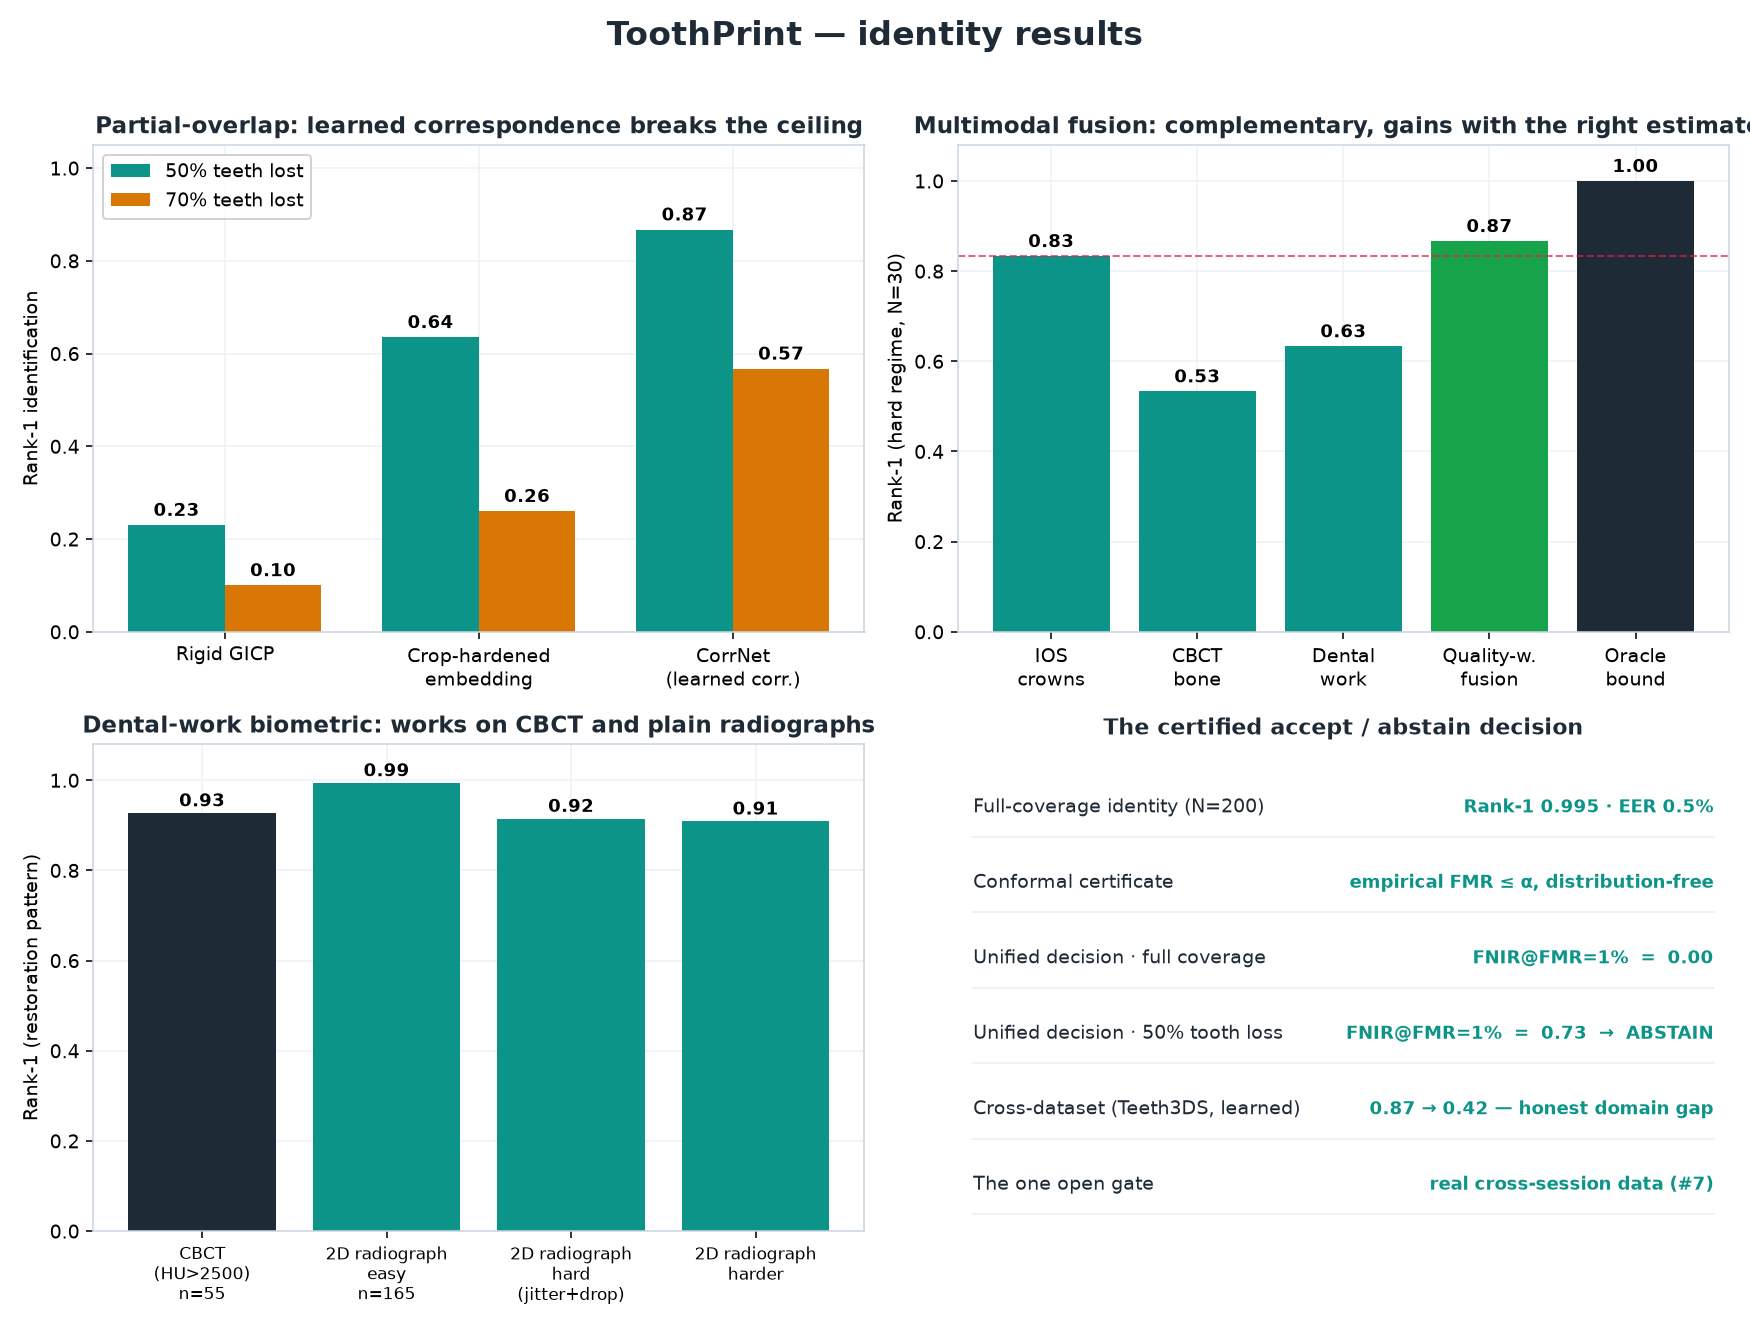
\includegraphics[width=\linewidth]{../docs/results_panel.png}
\caption{Headline results: partial-overlap breakthrough, fusion complementarity, dental-work across modalities, the certified decision.}\label{fig:panel}
\end{figure}

\begin{figure}[t]\centering
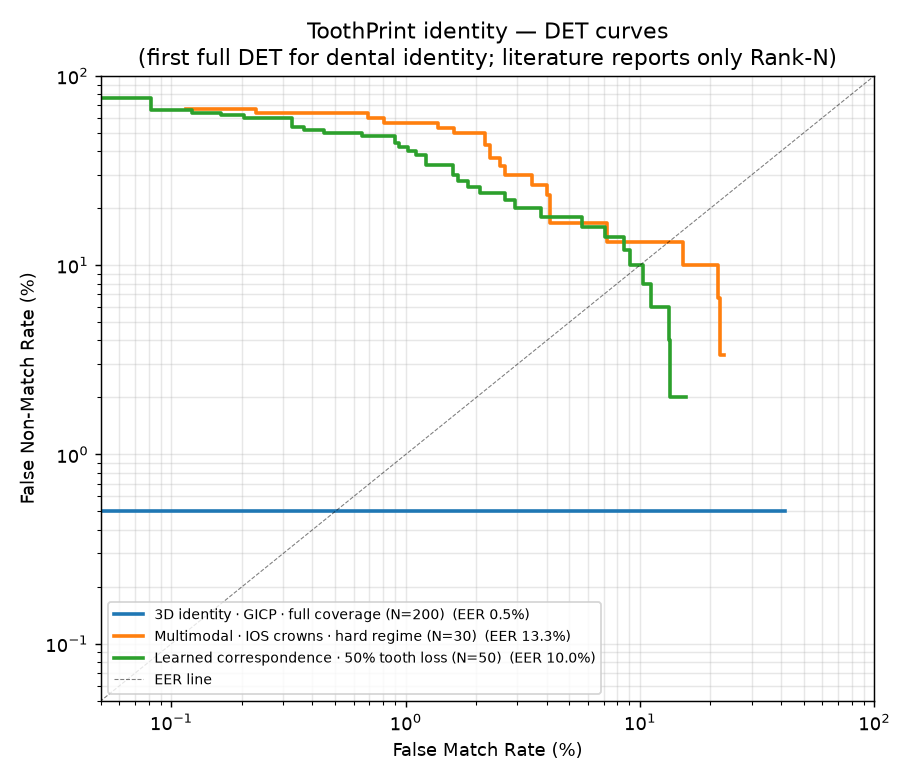
\includegraphics[width=0.92\linewidth]{../docs/det_curves.png}
\caption{Full DET curves per identity pillar (first for dental identity).}\label{fig:det}
\end{figure}

\section{Honest limitations}
\textbf{(1) Open-set collapses under partial overlap.} At keep-0.5 every method's FNIR@FMR=1\% is 0.74--0.87 (vs 0.03 full)---a half-arch fits many gallery arches, so impostor/genuine score tails overlap. Certified rejection is a near-full-coverage property; under heavy tooth loss the correct behaviour is to \textbf{abstain}. \textbf{(2) Cross-dataset domain gap.} CorrNet trained on Poseidon3D, run on Teeth3DS+, drops keep-0.5 $0.87\!\rightarrow\!\textbf{0.42}$ (still 34$\times$ chance, still $>$GICP); the learned descriptors are partly dataset-specific. \textbf{(3) Extreme tooth loss} (keep-0.3) is the hard tail (0.57 realistic). \textbf{(4) Fusion gain is Rank-1-only and small} (AUC regresses under naive weighting).

\section{The binding constraint: real cross-session data}
Every identity number here---CorrNet's 0.87, the 0.995, the Teeth3DS results---rests on \textbf{synthetic} re-scans/crops of single-timepoint arches, because no open dataset pairs the same person across visits with the needed modality. This is a \emph{data} limit no code closes. Until such data validates the pipeline, ToothPrint is \textbf{best-by-design and validated in simulation}, not proven on real longitudinal data---and the repository states this throughout.

\section{Reproducibility}
Datasets are gitignored; paths are env-configurable, reference baselines are read from committed artifacts, and committed synthetic fixtures run the 3D pipeline end-to-end with no off-machine data (\texttt{TOOTHPRINT\_FIXTURES=1}; see \texttt{REPRODUCE.md}).

\section{Conclusion}
ToothPrint is, to our knowledge, the most complete and most partial-overlap-robust \textbf{certified} dental-identity system demonstrable without gated longitudinal data: a learned correspondence matcher that quadruples rigid performance under 50\% tooth loss, a conformal accept/abstain certificate, a dental-work biometric across CBCT and radiographs, and a discipline of reporting the regimes where it must decline. The path to a clinical claim runs through real cross-session data, not more code.

\small
\textbf{References.}
Zhou et al. (2024), \emph{Bioengineering}---3D intraoral-scan identification.
Wang et al. (2019)---Dynamic Graph CNN (EdgeConv).
Deng et al. (2019/2020)---(Sub-centre) ArcFace.
Segal et al. (2009)---Generalised-ICP.
Vovk et al.---Conformal prediction.
Qin et al. (2022)---GeoTransformer.

\end{document}
